\documentclass[letterpaper,10pt,pagesize=pdftex,headings=normal]{scrreprt}
\setkomafont{section}{\large}
\setkomafont{subsection}{\normalsize}
\setkomafont{subsubsection}{\slshape}
\KOMAoptions{footnotes=multiple}
\usepackage[hang,flushmargin]{footmisc}
  % \addtolength{\skip\footins}{10pt}
  % \renewcommand\hangfootparskip{\baselineskip}
  \setlength{\footnotesep}{\baselineskip}
  \renewcommand\footnotelayout{\normalsize}
\usepackage[left=1in,right=1in,bottom=1in,top=1in,headsep=24pt]{geometry}
% \linespread{1.05} 
\renewcommand{\chapterheadstartvskip}{\vspace*{-\baselineskip}}
% \renewcommand*{\chapterheadendvskip}{\vspace{20pt}}
\usepackage{lastpage,scrpage2}
% \setkomafont{pagenumber}{}
\deftripstyle{harry}{}{}{\normalfont\sffamily\footnotesize c.~saitis: a survey of practices for crowdsourcing $\mid$ page \thepage~of \pageref*{LastPage}}{}{}{}
\pagestyle{harry}
\renewcommand{\chapterpagestyle}{harry}


\usepackage[T1]{fontenc}
\usepackage[utf8]{inputenc}
\usepackage[utopia]{mathdesign}
\usepackage{PTSans}
\usepackage{microtype}
\usepackage{textcomp}
\usepackage[inline]{enumitem}
\usepackage{graphicx}
\usepackage{booktabs,colortbl}
\usepackage{array}
\usepackage{multirow}
\usepackage{longtable}
\usepackage{tabu}
	% \setlength{\LTcapwidth}{0.9\textwidth}
\usepackage{colortbl}
\usepackage{tabularx}
\newcolumntype{L}{>{\raggedright\arraybackslash}X}
\newcolumntype{R}{>{\raggedleft\arraybackslash}X}

\usepackage[usenames,dvipsnames]{xcolor}
\definecolor{bleudefrance}{rgb}{0.19, 0.55, 0.91}
\definecolor{metablue}{rgb}{0.12, 0.48, 0.73}
\definecolor{awesome}{rgb}{1.0, 0.13, 0.32}
\usepackage{tikz}
\usepackage[colorlinks=true,allcolors=bleudefrance]{hyperref}
  \urlstyle{rm}


% BIBLIOGRAPHY SETUP 
\usepackage{natbib}
  % \def\bibfont{\footnotesize}
  \setlength{\bibhang}{0.5em}
  % \setlength{\bibsep}{0.4ex}

\titlehead{
  \fontsize{26}{10}\selectfont\sffamily\bfseries a survey of practices \\ for crowdsourcing
	}
\title{
	\raggedright\Large \textbf{Charalampos Saitis} \\ 
	\normalfont\sffamily\normalsize Distributed Digital Music Archives and Libraries Lab \\
	Schulich School of Music, McGill University
	}
\author{}
\date{}

\begin{document}
\maketitle
\tableofcontents

\chapter{Prelude}

Humans are critical components for performing quality control in a pattern recognition process, correcting the inevitable errors that automated systems make and ensuring these errors do not compound themselves in subsequent workflow steps \citep{hankinson2012b,burlet2012}. Correction, however, can be very time, labour and cost intensive. In the case of optical character recognition (OCR)---the textual counterpart of OMR---some unique solutions have been developed, leveraging collective intelligence and the Web to help offset the costs of this task. The reCAPTCHA project \citep{ahn2008} has produced over 5 billion human-corrected OCR words by presenting the correction task as a spam-fighting challenge to prove that the user is a human and not an automated system. The Australian Newspapers Digitisation Project \citep{holley2009} has created a distributed correction system, where more than 9,000 volunteers have now corrected more than 12.5 million lines of text, with more corrections added all the time.\\

\noindent Both these examples are manifestations of \textbf{crowdsourcing}, a Web-enabled, distributed problem-solving model that has emerged during the past decade \citep{brabham2013}. Its technical and conceptual underpinnings of crowdsourcing lie at the intersection of collective intelligence, outsourcing and the Internet \citep{brabham2013,saxton2013}. Crowdsourcing can be described as a \textbf{method} where a large number of people, known as contributors, are enlisted to help solve a problem defined by the system owners (corporations, libraries, researchers, etc.), which would normally require intensive (and often tedious), costly labour. Apart from helping reaching out to potentially thousands of users around the globe, the Internet offers a high degree of automation and unique possibilities for user management (e.g., wiki, discussion groups) \citep{doan2011}. Ever since the term was coined in 2006 \citep{howe2006}, many names (citizen science, crowd wisdom, human computation, etc.), definitions \citep{arolas2012} and typologies \citep{geiger2011} of crowdsourcing have appeared in an attempt to provide this new concept with a theoretical framework.\\

\begin{figure}[h]
\begin{center}
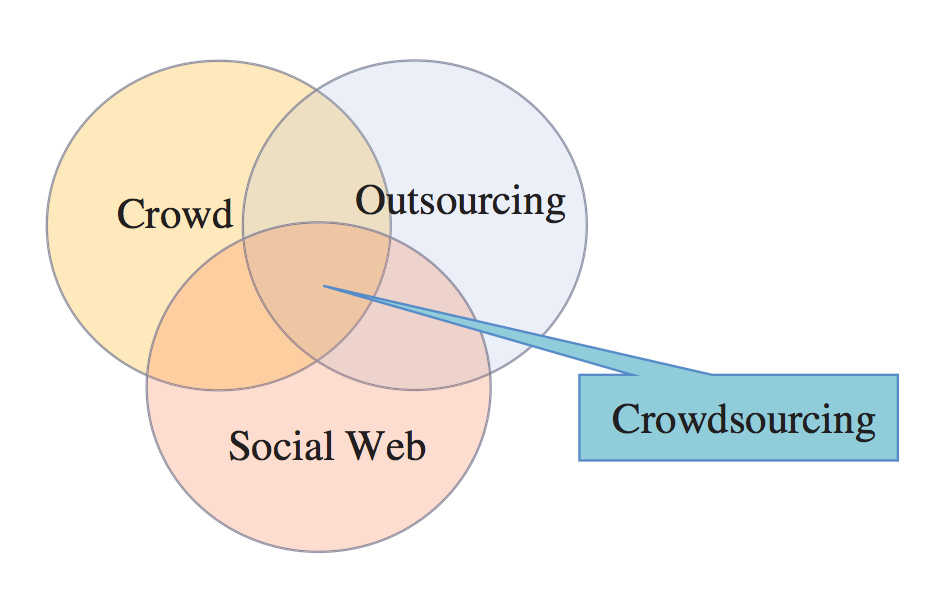
\includegraphics[scale=0.4]{figures/saxton13venn.png}
\caption{Conceptual underpinnings of crowdsourcing. From \citet{saxton2013}.}
\end{center}
\end{figure}

\chapter{Crowdsourcing in practice: Some examples}

\begin{longtabu} to\linewidth {@{}>{\hsize=.35\hsize}L >{\hsize=1.65\hsize}L}

\toprule 
Project & Description \\ 
  \midrule \endfirsthead
  
\multicolumn{2}{@{}l}{continued from previous page} \\
\midrule 
Project & Description \\ 
  \midrule \endhead 
  
\bottomrule \endlastfoot    
  
% \midrule
\multicolumn{2}{r@{}}{continued on next page} \endfoot

\href{http://www.innocentive.com/}{InnoCentive} & 
Crowdsourcing solution to problems defined by business, research, and social organizations through a cloud-based innovation management platform.
\\ \midrule

\href{http://www.ideastorm.com/}{IdeaStorm} by Dell & 
Dell is inviting people to identify ideas about computers and computer services that are most important and most relevant to the public.   
\\ \midrule

\href{http://www.nabuur.com/}{Nabuur} & 
From Wikipedia's entry: The Nabuur Foundation is a non-profit organization based in Giethoorn, Netherlands. It aims to help in the development of impoverished communities by enabling people from other countries to help the community members through Nabuur's website.
\\ \midrule

MicroPlace & 
A social business now owned by eBay. It facilitated peer-to-peer microfinance loans, but not on a charitable basis like its competitor Kiva.
\\ \midrule

CrowdSpirit & 
CrowdSpirit was an innovation community based on the idea of crowdsourcing the whole product development process, from ideation to distribution. A good example of what makes crowdsourcing \emph{not} work \citep{chanal2010}. 
\\ \midrule

\href{http://www.marketocracy.com/}{Marketocracy} & 
An online ``farm system'' for investors. Individual aspiring investors are invited to prove themselves/test their theories by managing a model portfolio in real time. The best managers are then allowed to apply their skills to client accounts.
\\ \midrule

\href{https://www.mturk.com/}{Mechanical Turk} &
A crowdsourcing platform/marketplace by Amazon. Launched in 2005. Businesses (known as Requesters) can post so-called Human Intelligence Tasks (HITs), setting a monetary compensation. Individuals (known as Workers) can then choose among existing HITs and complete them. HITs can be placed either through the Amazon Mechanical Turk API or directly on \url{https://requester.mturk.com/}.
\\ \midrule

\href{http://www.google.com/recaptcha/intro/}{reCAPTCHA} & 
The reCAPTCHA project \citep{ahn2008} produces human-corrected OCR words/human-labelled images by presenting the correction task as a spam-fighting challenge (CAPTCHA) to prove that the user is a human and not an automated system. It was acquired by Google in 2009. Currently used by Google Books, Google Maps and the New York Times archives among others. 
\\ \midrule

\href{http://www.istockphoto.com/}{iStockphoto} & 
A crowdsourced online marketplace for royalty-free stock images.
\\ \midrule

Spotting the Weedy Invasives & 
Volunteer identifying and mapping of invasive plants along hiking trails in the New York/New Jersey Highlands. Operated by Rutgers University and the New York/New Jersey Trail Conference and sponsored by the United States Department of Agriculture.
\\ \midrule

Invasive Plant Atlas of New England & 
Another project that invites volunteers to identify and map invasive plants (in New England).
\\ \midrule

ReClam the Bay & 
Community volunteers are engaged in restoring shellfish to Barnegat Bay, New Jersey. 
\\ \midrule

\href{https://www.gutenberg.org}{Project Gutenberg} & 
A book digitization and archival project where volunteers create and/or proofread digital versions of books (some formats: plain text, HTML, PDF, mobi). Founded in 1971 by Michael S.~Hart, Project Gutenberg is the oldest digital library. 
\\ \midrule

IBM's 2006 Innovation Jam &
In July 2006, IBM hold an online open-call brainstorming session for innovative business ideas. The event reportedly attracted more than 150,000 participants from 104 countries and 67 different companies over the course of two 72-hour sessions.\footnote{\url{http://www-03.ibm.com/ibm/history/ibm100/us/en/icons/innovationjam/}}
\\ \midrule

Cisco Systems' I-Prize  & 
An external innovation competition aimed to find the next major business opportunity for Cisco Systems. Run in 2007. 
\\ \midrule

\href{http://www.liveops.com/}{LiveOps} & 
Maintains a pool of crowdsourced call center agents.
\\ \midrule

\href{http://99designs.ca/}{99designs} & 
Maintains a pool of crowdsourced graphic designers. 
\\ \midrule

\href{https://twitter.com/snowtweets}{SnowTweets} & 
The project invites people to report their local snow depth measurements, which are then mapped and used by environmental researchers at the University of Waterloo, Canada. User measurements are reported through Twitter. Launched in 2009.
\\ \midrule

\href{http://fold.it/}{Foldit} & 
A computer game wherein players interactively reshape improperly folded protein structures in the direction they believe will lead to the highest score. The score increases as the energy of the structure decreases; the goal is to find the native state of the protein conformation \citep{cooper2010}.
\\ \midrule

\href{http://fossilfinder.coe.uga.edu/about/what-is-fossil-finders/}{Fossil Finders} & 
A project that brings together educators, students, and researchers from the University of Georgia and the Paleontological Research Institution in Ithaca, New York, to learn about Devonian-age fossils.
\\ \midrule

\href{http://www.galaxyzoo.org/}{Galaxy Zoo} &
Astronomy project which invited people to assist in the morphological classification of more than 900,000 galaxies by eye that had been imaged by the Sloan Digital Sky Survey at the Apache Point Observatory in New Mexico, USA. Launched in 2007, it led to the creation of Zooniverse.org, a framework to support and host citizen science projects. Various versions followed, which either asked for more detailed classifications, classified images of galaxies collected by other observatories/telescopes, or compared different datasets. 
\\ \midrule

\href{http://razor.sourceforge.net/}{Vipul's Razor} & 
(From the source:) Through user contribution, Razor establishes a distributed and constantly updating catalogue of spam in propagation that is consulted by email clients to filter out known spam. Detection is done with statistical and randomized signatures that efficiently spot mutating spam content.
\\ \midrule

The ESP Game & 
The Extra Sensory Perception (ESP) Game reveals the same image to two random players and asks each to guess what the other person has written to describe it. If they agree, that word or phrase is then used to annotate the picture. The same image is presented to multiple pairs of players until a detailed label is built up. It was originally developed by Luis von Ahn in 2003 \citep{ahn2004}. In 2006, Google bought a license to create its own version of the game, the Google Image Labeler, which run until 2011. 
\\ \midrule

helpfindjim.com & 
An open call to help find one Jim Gray.
\\ \midrule

\href{http://en.childrenslibrary.org/index.shtml}{International Children's Digital Library} & 
The ICDL Foundation is a nonprofit project that was created in 2003 by researchers at the University of Maryland at College Park. Its goal is to make the best in children's literature available online free of charge. Users contribute and/or translate books. ICDL currently\footnote{Website visited on December 3, 2014.} offers 4619 ebooks in 59 languages, complete with 2 iPhone/iPad apps; users (including contributors) come from 228 countries.
\\ \midrule

TagATune & 
TagATune is an audio-based online game that aims to extract descriptions of sounds and music from human players. The process is relatively similar to the ESP game, i.e., two independent players have to agree on a description for a given sound \citep{law2007}.
\\ \midrule

\href{http://projects.csail.mit.edu/soylent/}{Soylent} & 
From the source: Soylent is a word processor with a crowd inside: an add-in to Microsoft Word that uses crowd contributions to perform interactive document shortening, proofreading, and human-language macros. Underlying Soylent is a new programming design pattern called Find-Fix-Verify that splits tasks into a series of generation and review stages to control costs and increase quality. Paper: \citet{bernstein2010}.
\\ \midrule

\href{http://www.cs.umd.edu/hcil/monotrans/}{MonoTrans} & 
From the source: An iterative protocol in which monolingual human participants work together to improve imperfect machine translations.
\\ \midrule


Kasparov versus the World & 
An Internet-based chess game played in 1999 between Garry Kasparov and a ``world team'' comprised over 50,000 people from more than 75 countries who decided on moves by plurality vote (Wikipedia entry).
\\ \midrule


\href{http://www.vizwiz.org/}{VizWiz} & 
A free talking iPhone app that enables blind and visually impaired users to receive quick answers to questions about their surroundings. It combines automatic image processing, anonymous web workers (through an abstraction layer on top of the Amazon Mechanical Turk API), and members of the user's social network in order to collect fast and accurate responses. 
\\ \midrule

\href{http://www.chacha.com/}{ChaCha} & 
Wikipedia entry: ChaCha is a human-guided search engine. It provides free, real-time answers to any question, through its website, or by using one of the company's mobile apps. From the source: It is used primarily as a marketing tool for brand advertisers to reach and engage with their target audience in real-time.
\\ \midrule

\href{http://www.nla.gov.au/content/newspaper-digitisation-program}{The Australian Newspapers Digitisation Project} & 
Ongoing program that is digitising historic Australian newspapers from 1803 onwards using OCR. To improve and enhance the quality of the data, the public is correcting OCR transcriptions and/or adding tags to full-text articles. The program forms part of the larger \href{http://trove.nla.gov.au/}{Trove} project by the National Library of Australia. 
\\ \midrule

\href{http://menus.nypl.org/}{What's on the menu?} & 
The New York Public Library is inviting people to help improve its historical restaurant menu collection by transcribing the menus, dish by dish.
\\ \midrule

\href{http://blogs.ucl.ac.uk/transcribe-bentham/}{Transcribe Bentham} & 
A public collaborative transcription initiative at the University College London to support the creation of a vast digital repository of Jeremy Bentham's writings. Users are asked to transcribe text and encode their transcriptions in TEI-compliant XML (Text Encoding Initiative).
\\ \midrule

\href{http://www.whats-the-score.org/}{What's the score at the Bodleian?} & 
Ongoing music score annotation project which invites people to describe newly digitized scores of the Bodleian Libraries at the University of Oxford (UK), mostly piano music from the nineteenth century. Uses the Zooniverse interface/platform. 
\\ \midrule

\href{http://www.oldweather.org/}{Old Weather} & 
Crowdsourcing transcriptions of handwritten text from historical ship logs to improve reconstructions of past weather and climate. Contributors can provide new transcriptions or correct computer-transcribed (OCR) ones. Uses the Zooniverse interface/platform.
\\ \midrule

\href{http://www.kulturarv.dk/1001fortaellinger/en_GB}{1001 Stories Denmark} & 
A collection/website of about 1001 cultural heritage sights in Denmark. End-users are invited to contribute by adding/recommending new places, tagging/commenting on existing stories, or uploading images and videos.
\\ \midrule

\href{http://beeldengeluidwiki.nl/index.php/Hoofdpagina}{Netherlands Institute for Sound and Vision wiki} & 
Volunteer contribution of contextual information on Dutch television programmes, broadcasters, presenters, etc.
\\ \midrule

\href{http://sounds.bl.uk/Sound-Maps/UK-Soundmap}{UK\_Soundmap} & 
The British Library invited people to capture ``sounds of today'' through using the mobile pp Audioboo. Sound clips are uploaded together with some metadata such as geo-coordinates, which help place them on an interactive map and make them searchable.
\\ \midrule

\href{https://www.wir-waren-so-frei.de/}{Wir Waren So Frei} & 
The Deutsche Kinemathek and the Bundeszentrale für politische Bildung created an archive of visual testaments to the fall of the Berlin Wall through inviting the public to contribute photographs, films, and the stories behind them. 
\\ \midrule

\href{http://www.massobs.org.uk/}{Mass Observation Project} & 
The original Mass Observation project was started in 1937 by a group of people who aimed to record everyday life in Britain. To this purpose, they recruited voluntary observers/writers. This work continued until the early 1950s. In 1981, a new public call was launched, continuing until today. 
\\ \midrule

Civil War Phases & 
The Library of Congress published a rare collection of Civil War photographs on flickr and invited people to identify soldiers and/or photographers.\footnote{\url{https://www.flickr.com/photos/library_of_congress/sets/72157625520211184/}}
\\ \midrule

\href{https://github.com/beeldengeluid/waisda}{Waisda?} & 
A Web-based game developed by the Netherlands Institute for Sound and Vision, KRO broadcasting, and VU University Amsterdam wherein players annotate television heritage. Similar to ESP, players gain points if they guess correctly what their opponent has written within a given amount of time.  
\\ \midrule

\href{http://emotify.org/}{Emotify} & 
A Web-based (standalone or as a Facebook app) game wherein players describe induced emotions (up to three from a list of nine) upon listening to one-minute music fragments \citep{aljanaki2014}.
\\ \midrule

\href{http://www.hookedonmusic.org.uk/}{Hooked} & 
A game that collects ``hook'' (``the most salient, easiest-to-recall fragment in a piece of music'') and ``catchiness'' (``the long-term musical salience'') data for music songs from its players through three tasks: recognition (listen to random excerpt and recognize within a few seconds), verification (sing along recognized tune), and prediction (find catchier excerpt) \citep{burgoyne2013}. 
\\ \midrule

Click! &
``Click! A Crowd-Curated Exhibition'' was launched by the Brooklyn Museum in 2008. The museum first invited photographers to submit electronically images that responded to the theme ``The Changing Faces of Brooklyn.'' The general public was then invited to assess the submissions online through a custom built evaluation tool. 
\\ \midrule

\href{https://www.kaggle.com/}{Kaggle} &
Crowd-sourced data prediction. Companies, organizations, and researchers post their data and data analysts from all over the worlds are invited to compete for finding the best model(s).
\\ \midrule

\href{https://www.indabamusic.com/}{Indaba Music} &
From \citet{gomes2012}: It allows to create, edit and mix music collaboratively. Crowds of people from anywhere in the world can collectively produce music without having to be professionals in the area.
\\ \midrule

\href{http://www.queremos.com.br/}{Queremos!} &
Translated from the source: Queremos! (We want!) is an innovative platform [in Brazil] that connects fans, artists and producers to promote shows. The initiative comes from the crowd itself (fans), based on which artist(s) they ``want!'' 
\\ \midrule

\href{http://picktheband.com/}{PickTheBand.com} &
From \citet{gomes2012}: It allows fans to participate in decisions made by their favorite artists. From the source: ``The world's first fan run label.'' 
\\ \midrule

\href{https://www.voices.com/}{Voices.com} &
An online marketplace for voice overs: Maintains a pool of crowdsourced ``voices'' and voice-over jobs. 
\\ \midrule

Askville &
A user-driven research site founded by Amazon and run between 2006 to 2013. Unlike other crowdsourced Q\&A initiatives, Askville was designed with game characteristics (with a point system based on asking/answering questions). It also provided discussion boards.
\\ \midrule

\href{http://www.webook.com/}{webook.com} &
An online platform for writers, readers and literary agents geared towards discovering new writers and helping them get published.
\\ \midrule

\href{https://www.lendingclub.com/}{Lending Club} &
From Wikipedia: Lending Club operates an online lending platform that enables borrowers to obtain a loan, and investors to purchase notes backed by payments made on loans.
\\ \midrule

\href{http://www.angieslist.com/}{Angie's list} &
Crowd-sourced reviews of local businesses.
\\ \midrule

\href{https://www.lulu.com/}{Lulu} &
From Wikipedia: An online print-on-demand, self-publishing and distribution platform.
\\ \midrule

\href{http://inklingmarkets.com/}{inkling markets} &
From the source: Inkling offers crowdsourced forecasting applications and solutions to help organizations improve their decision making through more accurate forecasts and greater internal transparency.
\\ \midrule

\href{https://en.eyeka.com/}{eYeka} &
From the source: eYeka is a crowdsourcing platform that connects creative individuals with brands to boost their return on marketing investment.
\\ \midrule

\href{http://opendata.paris.fr/page/home/}{OpenDataParis} &
An open data project by the Mayor of Paris to enable citizen participation in urban issues such as accessibility and bicycle parking.
\\ \midrule

\href{http://www.stayingalive.org/en.php}{Staying Alive} &
Formerly known as Arrêt Cardiaque, Staying Alive is a mobile app mapping defibrillators worldwide and allowing users to report new ones.
\\ \midrule

\href{http://seeclickfix.com/}{SeeClickFix} &
A Web tool for community activism. Citizens can publicly report neighborhood issues to appropriate services such as local government.
\\ \midrule

\href{https://www.elance.com/}{Elance} &
From \citet{nakatsu2014}: An online employment platform. Using Elance, a requestor can solicit work (e.g., design a website, write a program, create a marketing plan) from qualified professionals throughout the world who bid to be hired. 
\\ \midrule

Mark the Spot by AT\&T &
A mobile app that enables AT\&T customers to submit wireless coverage problems in real time, together with location information.
\\ \midrule

\href{http://curetogether.com/}{CureTogether} &
From \citet{nakatsu2014}: A website where patients with medical conditions can report on the performance of treatments they received. By gaining access to the millions of ratings reported to the website, patients can learn from the experiences of other patients with the same medical condition.
\\ \midrule

\href{http://www.40fires.org/}{40 Fires Foundation} &
An open source hardware design project by Riversimple. The company has published the design schematics of their hydrogen-powered car under a Creative Commons Attribution-Noncommercial license, inviting the public to take part in the design process.
\\ \midrule

\href{http://www.mob4hire.com/}{Mob4Hire} &
Crowd-sourced mobile app testing services and market research. It enables collaboration between developers and professional users who evaluate app usability under a fixed-fee structure.
\\ %\midrule

\end{longtabu}


\chapter{Definitions}\label{definitions}

\tabulinesep=1ex
\begin{longtabu} to\linewidth {@{}>{\hsize=0.4\hsize}L >{\hsize=1.6\hsize}L}

\toprule 
Source & Definition  \\ 
  \midrule \endfirsthead
  
\multicolumn{2}{@{}l}{continued from previous page} \\
\midrule 
Source & Definition \\ 
  \midrule \endhead 
  
\bottomrule \endlastfoot    
  
% \midrule
\multicolumn{2}{r@{}}{continued on next page} \endfoot  

\citet{howe2006,howe2008} & Crowdsourcing is the act of taking a task traditionally performed by a designated agent (such as an employee or a contractor) and outsourcing it by making an open call to an undefined but large group of people. Crowdsourcing allows the power of the crowd to accomplish tasks that were once the province of just a specialized few. Or to put it another way, crowdsourcing is to take the principles which have worked for open source software projects and apply them right across the entire spectrum of the business world.\footnote{On his crowdsourcing website/blog (\url{http://www.crowdsourcing.com/}) Howe rearranges this definition in two ``versions:''
\begin{itemize}
\item \textbf{The White Paper Version:} Crowdsourcing is the act of taking a job traditionally performed by a designated agent (usually an employee) and outsourcing it to an undefined, generally large group of people in the form of an open call. 
\item \textbf{The Soundbyte Version:} The application of Open Source principles to fields outside of software. 
\end{itemize}} \\

\midrule

\citet{brabham2013} & Crowdsourcing is an online, distributed problem-solving and production model ...  It is a model capable of
aggregating talent, leveraging ingenuity while reducing the costs and time formerly needed to solve problems.\footnote{Brabham draws a line between (what he defines as) crowdsourcing and such massive online participatory phenomena as Wikipedia and Linux. For Brabham, crowdsourcing combines traditional top-down production with bottom-up user production: ``the locus of control is between organization and online community.'' Wikipedia and Linux lack the former: contributors are not told what articles/code to create.} \\

\midrule

\citet{geerts2009} & Crowdsourcing is the online outsourcing of a task to (a group of) private individuals in the form of an open call. \\

\midrule

\citet{erickson2011} & Tapping the perceptual, cognitive or enactive abilities of many people to achieve a well-defined result such as solving a problem, classifying a data set, or producing a decision. \\

\midrule

\citet{doan2011} & A system is a crowdsourcing system if it enlists a crowd of humans to help solve a problem defined by the system owners, and if in doing so, it addresses the following four fundamental challenges: How to recruit and retain users? What contributions can users make? How to combine user contributions to solve the target problem? How to evaluate users and their contributions? \\

\midrule

\citet{geiger2012} & Crowdsourcing information systems are a special case of information systems that produce informational products and/or services for internal or external customers by harnessing the potential of crowds.\footnote{Here the authors built on the definition of information systems (IS) as work systems proposed by \citet{alter2008}: ``an IS is a system in which human participants and/or machines perform work (processes and activities) using information, technology, and other resources to produce informational products and/or services for internal or external customers.''} \\

\midrule

\citet{arolas2012} & Crowdsourcing is a type of participative online activity in which an individual, an institution, a non-profit organization, or company proposes to a group of individuals of varying knowledge, heterogeneity, and number, via a flexible open call, the voluntary undertaking of a task. The undertaking of the task, of variable complexity and modularity, and in which the crowd should participate bringing their work, money, knowledge and/or experience, always entails mutual benefit. The user will receive the satisfaction of a given type of need, be it economic, social recognition, self-esteem, or the development of individual skills, while the crowdsourcer will obtain and utilize to their advantage what the user has brought to the venture, whose form will depend on the type of activity undertaken.\footnote{Estellés-Arolas and de Guevara derived this definition through textual analysis of 40 definition-like descriptions of crowdsourcing extracted from 203 publications in ACM, IEEE, ScienceDirect, SAGE, and Emerald. The authors identified 8 characteristics which were then integrated into a more overarching definition:
\begin{enumerate*}[label=\alph*\upshape)]
\item there is a clearly defined crowd;
\item there exists a task with a clear goal;
\item the recompense received by the crowd is clear;
\item the crowdsourcer is clearly identified;
\item the compensation to be received by the crowdsourcer is clearly defined;
\item it is an online assigned process of participative type;
\item it uses an open call of variable extent;
\item it uses the internet.
\end{enumerate*}
An attempt to verify this integrated definition through 11 Internet-based projects such as Wikipedia and Threadless is also reported (see Table 4, page 197). 
} \\

\midrule

\citet{lebraty2013} & Crowdsourcing is the externalization by an organization, via an application using the Internet protocol, of an activity to a large number of individuals whose identities are most often anonymous. \\ 

\midrule

\citet{saxton2013} & Crowdsourcing is a sourcing model in which organizations use predominantly advanced internet technologies to harness the efforts of a virtual crowd to perform specific organizational tasks. \\

\midrule

\citet{pedersen2013} & A collaboration model enabled by people-centric web technologies to solve individual, organizational, and societal problems using a dynamically formed crowd of interested people who respond to an open call for participation. \\

\midrule

\citet{nakatsu2014} & We define crowdsourcing as a four-step process in which: \linebreak
(1) a requestor (either an individual or organization) identifies a specific task to be performed or problem to be solved; \linebreak
(2) the requestor broadcasts the task or problem online; \linebreak
(3) the crowd performs the task or solves the problem; \linebreak
(4) depending on the nature of the task, the requestor either \linebreak
-- (4a) sifts through the solutions and selects the best solution (selective crowdsourcing), or \linebreak
-- (4b) aggregates/synthesizes the crowd’s submissions in a meaningful way (integrative crowdsourcing). \\

\midrule

Merriam-Webster.com & Crowdsourcing is the practice of obtaining needed services, ideas, or content by soliciting contributions from a large group of people and especially from the online community rather than from traditional employees or suppliers.\footnote{The Wikipedia entry for ``crowdsourcing'' cites this definition.} \\

\end{longtabu}


\chapter{Describing crowdsourcing: Typologies and taxonomies}


% \tabulinesep=1ex
\begin{longtabu} to\linewidth {@{}>{\hsize=0.3\hsize}L >{\hsize=1.75\hsize}L >{\hsize=0.95\hsize}L}

\toprule 
Source & Description & Examples \\ 
  \midrule \endfirsthead
  
\multicolumn{3}{@{}l}{continued from previous page} \\
\midrule 
Source & Description & Examples \\ 
  \midrule \endhead 
  
\bottomrule \endlastfoot    
  
% \midrule
\multicolumn{3}{r@{}}{continued on next page} \endfoot


\multirow{2}{\hsize}{\citet{surowiecki2004}} & \textbf{Types of problems that can affect \emph{collective intelligence}}\footnote{\citet{nakatsu2014}: ``Predates the crowdsourcing literature by a few years, but provides a useful framework for studying problems solved by a crowd.''} & \\
\cmidrule(l){2-3}
& \parbox{\hsize}{
\begin{itemize}[leftmargin=*,nosep]
\item \emph{Cognition problems} (problems that have a definitive solution)
\item \emph{Coordination problems} (requires the crowd to coordinate their behaviour with one another)
\item \emph{Cooperation problems} (involve getting people to collaborate and work jointly together)
\end{itemize}} & \\

\arrayrulecolor{black}\midrule

\multirow{6}{\hsize}{\citet{howe2008}} & \textbf{\emph{What the crowd-}} & \\
\cmidrule(l){2-3}
& \emph{-knows}: Use and application of collective intelligence \linebreak
Subtypes: prediction markets, crowdcasting, brainstorming\linebreak
Further subtype \citep{geerts2009}: crowdcasting/storming hybrid & InnoCentive (crowdcasting), IdeaStorm (brainstorming), Nabuur (hybrid)\\ 
\arrayrulecolor{black!20}\cmidrule(l){2-3}
& \emph{-creates}: Production of mass creative works \linebreak Subtypes \citep{geerts2009}: product (all contributions are combined), market (contributions are used in a p2p form) & Wikipedia (product), Threadless (market)\\
\cmidrule(l){2-3}
& \emph{-thinks}: Filtering and organizing of vast information stores & Amazon, Threadless (consumer reviews/ratings) \\
\cmidrule(l){2-3}
& \emph{-funds}: Use of the crowd's collective pocketbook \linebreak Subtypes \citep{geerts2009}: product (all contributions are combined), market (contributions are used in a p2p form) & Kickstarter (product), MicroPlace (market) \\

\arrayrulecolor{black}\midrule

\multirow{3}{\hsize}{\citet{vukovic2009}} & \textbf{Two primary dimensions} & \\
\cmidrule(l){2-3}
& Mode (competition / marketplace) & Threadless (competition), CrowdSpirit (marketplace), Marketocracy (competition), Mechanical Turk (marketplace) \\
\arrayrulecolor{black!20}\cmidrule(l){2-3}
& Function (design and innovation / development and testing / marketing and sales / support) & Threadless (design and innovation), CrowdSpirit (development and testing), Marketocracy (marketing and sales), Mechanical Turk (support) \\

\arrayrulecolor{black}\midrule

\multirow{4}{\hsize}{\citet{corney2009}} & \textbf{Three dimensions} & \\
\cmidrule(l){2-3}
& Nature of the task (creation / evaluation / organisation) & InnoCentive (creation), market surveys (evaluation), reCAPTCHA (organisation) \\
\arrayrulecolor{black!20}\cmidrule(l){2-3}
& Nature of the crowd (any individual / most people / experts) & reCAPTCHA (any individual), iStockphoto (most people), InnoCentive (experts)\\
\cmidrule(l){2-3}
& Nature of the payment (contribution: voluntary / rewarded with a bonus or prize / rewarded at a flat rate) & iStockphoto (prize), reCAPTCHA (voluntary), InnoCentive (flat rate)\\

\arrayrulecolor{black}\midrule

\multirow{2}{\hsize}{\citet{geerts2009}} & \textbf{Attributes of crowdsourcing}\footnote{These theoretical attributes are grouped into three categories representing design propositions according to the so-called CIMO-logic: ``in this class of problematic Contexts, use this Intervention type to invoke these generative Mechanism(s), to deliver these Outcome(s)'' \citep[p.~395]{denyer2008}. Mechanism attributes are not included as Geerts considers them to be mainly based on empirical confirmation.} & \\
\cmidrule(l){2-3}
& \parbox{\hsize}{
\begin{itemize}[leftmargin=*,nosep]
\item Intervention attributes
  \begin{itemize}[leftmargin=*,nosep]
  \item Role of the company (mediator / own initiative)
  \item Type of participation (voting; rating; commenting; forum; weblog; social network; wiki; upload; financial)
  \item Party that takes initiative (crowd initiative / company initiative)
  \item Whose contributions are used (individual / crowd / combination / p2p)
  \item Financial rewards (yes / no)
  \item Interaction (yes / no)
  \item Input control (contributions not public; type of participation; screening; registration)
  \item Output control (company / crowd)
  \item Intellectual Property (company / crowd / public / not relevant)
  \end{itemize}
\item Context attributes
  \begin{itemize}[leftmargin=*,nosep]
  \item Phase (concept; development/design; testing; customer service; production; decision making; support)
  \item Field (science; design; consumer goods; music; journalism)
  \end{itemize}
\item Outcome attributes
  \begin{itemize}[leftmargin=*,nosep]
  \item Size and activity of crowd
  \item Composition participants
  \item Number and quality of contributions
  \item Company effort
  \end{itemize}
\end{itemize}} & \\



\arrayrulecolor{black}\midrule

\multirow{4}{\hsize}{\citet{bonney2009}} & \textbf{Three types of public participation in scientific research} & \\
\cmidrule(l){2-3}
& \emph{Contributory projects} (members of the public primarily contribute data) & Spotting the Weedy Invasives \\
\arrayrulecolor{black!20}\cmidrule(l){2-3}
& \emph{Collaborative projects} (members of the public contribute data but also may help to refine project design, analyze data, or disseminate findings) & Invasive Plant Atlas of New England \\
\cmidrule(l){2-3}
& \emph{Co-created projects} (designed by scientists and members of the public working together; at least some of the public participants are actively involved in most or all steps of the scientific process) & ReClam the Bay \\


\arrayrulecolor{black}\midrule

\multirow{2}{\hsize}{\citet{zwass2010}} & \textbf{Taxonomic framework of factors in \emph{co-creation}} & \\
\cmidrule(l){2-3}
& \parbox{\hsize}{
\begin{itemize}[leftmargin=*,nosep]
\item Performers (the world, prequalified individuals, community members, skilled contributors) 
\item Motivation (altruistic desire to contribute, passion, inner need to reciprocate, enjoyment / state of flow / playfulness, self-expression, identity construction, forming personal relationships, community norms, competitive spirit, learning, satisfying one's affiliation needs, self-esteem and self-efficacy, thymotic strivings, acquiring social capital and peer recognition, career advancement, own use, nonmonetary rewards, signaling, financial rewards)\footnote{Some of these terms are further explained in Table 1, page 29 of the source.} 
\item Governance (individual autonomy, collective norms, software code, facilitators, adhocracy, bureaucracy, market mechanism, hybrid forms)  
\item Task characteristics (structural complexity, intellectual demands, effort intensity, time frame) 
\item Product aggregation (searchable corpus, hyperlinking, progressive refinement, statistical ratings and rankings, competitions and voting, information markets, bottom-up taxonomy, moderators / auditors / facilitators) 
\item Economic beneficiary (the world, the community, the sponsoring firm, the aggregator, the contributors)
\end{itemize}} & \\ 

\arrayrulecolor{black}\midrule

\multirow{4}{\hsize}{\citet{rouse2010}} & \textbf{Three dimensions}\footnote{A taxonomy based on these dimensions is proposed in Fig.~1 of the source.} & \\
\cmidrule(l){2-3}
& Distribution of benefits (community / individualistic) & Project Gutenberg (community), Threadless (individualistic), Cisco Systems' 2007 I-Prize (individualistic) \\
\arrayrulecolor{black!20}\cmidrule(l){2-3}
& Supplier capabilities/Nature of the task (simple / moderate / sophisticated) & Project Gutenberg (simple), Threadless (moderate), Cisco Systems' 2007 I-Prize (sophisticated)\\
\cmidrule(l){2-3}
& Forms of motivation (\emph{intrinsic}: social status, altruism, personal achievement and learning; \emph{extrinsic}: self-marketing, instrumental, token compensation, market compensation)
& \\



\arrayrulecolor{black}\midrule

\multirow{2}{\hsize}{\citet{malone2010}} & \textbf{Describing the goals and design of a \emph{collective intelligence system} through four main questions} & \\
\cmidrule(l){2-3}
& \parbox{\hsize}{
\begin{itemize}[leftmargin=*,nosep]
\item \emph{What is being done?} [Goal] (create / decide) 
\item \emph{Who is doing it?} [Staffing] (crowd / hierarchy or management) 
\item \emph{Why are they doing it?} [Incentives] (money / love / glory)
\item \emph{How are they doing it?} [Structure/Process]
  \begin{itemize}[leftmargin=*,nosep]
  \item How -- create (collection / collaboration)
  \item How -- decide (group decision / individual decisions)
  \end{itemize}
\end{itemize}} & \\


\arrayrulecolor{black}\midrule

\multirow{5}{\hsize}{\citet{geiger2011}} & \textbf{Four characteristics} & \\
\cmidrule(l){2-3}
& Preselection of contributors (qualification-based / context-based / both / none) & iStockphoto (qualification-based), InnoCentive (context-based), LiveOps (both), reCAPTCHA (none) \\
\arrayrulecolor{black!20}\cmidrule(l){2-3} 
& Accessibility of peer contributions (modify / assess / view / none) & Wikipedia (modify), iStockphoto (assess), 99designs (view), reCAPTCHA (none) \\
\cmidrule(l){2-3}
& Aggregation of contributions (integrative / selective) & reCAPTCHA (integrative), InnoCentive (selective), Wikipedia (integrative), iStockphoto (integrative) \\
\cmidrule(l){2-3}
& Remuneration for contributions (fixed / success-based / none) & LiveOps (fixed), InnoCentive (success-based), iStockphoto (success-based), reCAPTCHA (none) \\

\arrayrulecolor{black}\midrule

\multirow{6}{\hsize}{\citet{wiggins2011}} & \textbf{Five types of \emph{citizen science}} & \\
\cmidrule(l){2-3} 
& \emph{Action} (encourage participant intervention in local concerns; employ participatory action research approaches mostly based on ``bottom-up'' organizing) & ReClam the Bay \\
\arrayrulecolor{black!20}\cmidrule(l){2-3}
& \emph{Conservation} (volunteer engagement focuses on data collection activities; include explicit educational goals or content) & Invasive Plant Atlas of New England \\
\cmidrule(l){2-3}
& \emph{Investigation} (focused on scientific research goals requiring data collection from the physical environment; education not always an explicit goal; range in score from regional to international) & SnowTweets\\
\cmidrule(l){2-3}
& \emph{Virtual} (similar to Investigation but all project activities are ICT-mediated with no physical elements whatsoever) & Foldit \\
\cmidrule(l){2-3}
& \emph{Education} (primary objectives are education and outreach) & Fossil Finders \\

\arrayrulecolor{black}\midrule

\multirow{10}{\hsize}{\citet{doan2011}} & \textbf{Classification along nine dimensions} & \\
\cmidrule(l){2-3}
& Nature of collaboration (explicit / implicit) & Wikipedia (explicit), reCAPTCHA (implicit) \\
\arrayrulecolor{black!20}\cmidrule(l){2-3}
& Target problems (evaluating / sharing / building artifacts / networking / other) 
& Threadless (evaluating), Galaxy Zoo (sharing), Wikipedia (building), LinkedIn (networking), reCAPTCHA (other)
\\
\cmidrule(l){2-3}
& How to recruit and retain users\footnote{\label{chal}These dimensions correspond to the fundamental challenges that a crowdsourcing system should address according to the authors' definition (see Sec.~\ref{definitions} and Sec.~\ref{framework}).} (require users\footnote{If one has the authority to do so. For example, students may be asked to execute a task as part of their course requirements.} / pay users / ask for volunteers / make users pay for service / piggyback on user traces) & Mechanical Turk (pay), Wikipedia (ask), reCAPTCHA (make pay for service), Google (piggyback) \\
\cmidrule(l){2-3}
& What can users do\textsuperscript{\ref{chal}} (explicit: review; vote; tag; share knowledge; build software / implicit: play games with a purpose; solve CAPTCHAs; keyword search; browse Web sites) \linebreak 
$\rightarrow$ Need to consider: cognitive demand, impact of a contribution, machine contributions (e.g., correcting OCR/OMR transcriptions), user interface design 
& Amazon (review), Threadless (vote), del.icio.us (tag), Galaxy Zoo (share knowledge), Linux (build software), ESP (gamification), reCAPTCHA, Google \\ 
\cmidrule(l){2-3}
& How to combine user input\textsuperscript{\ref{chal}} (loosely $\leadsto$ tightly) & tagging (loosely), Wikipedia (tightly), Amazon (reviews are not combined but ratings are) \\ 
\cmidrule(l){2-3}
& How to evaluate user input\textsuperscript{\ref{chal}} (manually: monitoring by system owners or distributed among trusted users / automatic: machine tests) & \\
\cmidrule(l){2-3}
& Degree of manual effort (little $\leadsto$ substantial) \linebreak 
$\rightarrow$ Need to consider: how much the system is automated, how to divide the manual effort between the users and the system owners
& combine ratings (little), combine code (substantial) \\
\cmidrule(l){2-3}
& Role of human users (slaves / perspective providers / content providers / component providers)
& reCAPTCHA (slaves), Flickr (content), Wikipedia (slaves, perspective, content) \\
\cmidrule(l){2-3}
& Architecture (standalone / piggyback) & Wikipedia (standalone), reCAPTCHA (piggyback) \\

\arrayrulecolor{black}\midrule

& & \\
& & \\

\multirow{3}{\hsize}{\citet{schenk2011}} & \textbf{Two basic dimensions} & \\
\cmidrule(l){2-3}
& Nature of the process (integrative / selective) & Wikipedia (integrative), Threadless (selective)\\
\arrayrulecolor{black!20}\cmidrule(l){2-3}
& Task complexity (simple / complex / creative) & Wikipedia (complex), Threadless (creative) \\



\arrayrulecolor{black}\midrule

\multirow{2}{\hsize}{\citet{yuen2011}} & \textbf{Categorization based on four characteristics} & \\
\cmidrule(l){2-3}
& \parbox{\hsize}{
\begin{itemize}[leftmargin=*,nosep]
\item Application (voting system / information sharing system / game / creative system)
\item Algorithm
\item Dataset
\item Performance (user participation; quality management; cheating detection) 
\end{itemize}
$\rightarrow$ user participation factors: demographics, financial incentives, intrinsic incentives, worker behavior
}
& Vipul's Razor (voting), Wikipedia (information sharing), ESP (game), Threadless (creative) \\


\arrayrulecolor{black}\midrule

\multirow{5}{\hsize}{\citet{erickson2011}} & \textbf{Four types of crowdsourcing based on a space-time four quadrant model}\footnote{Adapted from the CSCW (Computer Supported Cooperative Work) spatial and temporal quadrants \citep[cf.][]{nichols1997}.} & \\
\cmidrule(l){2-3}
& \emph{Audience-centric}---same time/place & digital audience backchannels \\
\arrayrulecolor{black!20}\cmidrule(l){2-3}
& \emph{Event-centric}---same time/different places  & innovation jams \\
\cmidrule(l){2-3}
& \emph{Geocentric}---different times/same place & FourSquare \\
\cmidrule(l){2-3}
& \emph{Global}---different times/places & Wikipedia, ESP \\

\arrayrulecolor{black}\midrule

\multirow{2}{\hsize}{\citet{bratvold2011}} & \textbf{A taxonomy based on the relationship of the worker to the work}\footnote{Bratvold claims that ``when we consider grouping crowdsourcing into the relationship of the worker to the work (rather than outputs), it becomes much easier to segment into a handful of divisions that survive very well through time.''} & \\
\cmidrule(l){2-3}
& \parbox{\hsize}{
\begin{itemize}[leftmargin=*,nosep]
\item Microtasks (employ workers to perform individual [micro] tasks without regard to the entire project)
\item Macrotasks (workers can see more, if not all, of the project and get involved with the portion they are knowledgeable in)
\item Crowdfunding (classifies companies that employ crowds to provide work in the form of monetary donations)
\item Contests (asking a crowd for work and only providing compensation to the chosen entries)
\end{itemize}} & \\

\arrayrulecolor{black}\midrule

& & \\
& & \\

\multirow{7}{\hsize}{\citet{quinn2011}} & \textbf{Classification along six dimensions} & \\
\cmidrule(l){2-3}
& Motivation (pay; altruism; enjoyment; reputation; implicit work) & Mechanical Turk (pay), helpfindjim.com (altruism), ESP (enjoyment), ICDL (reputation), reCAPTCHA (implicit work) \\
\arrayrulecolor{black!20}\cmidrule(l){2-3}
& Quality control (output agreement; input agreement; economic models;\footnote{Adopt compensation schemes that elicit more good-quality contributions for less reward \citep[e.g., ``quota'' systems,][]{mason2009}.} defensive task design;\footnote{Design tasks so that cheating is obvious or impossible.} redundancy; statistical filtering;\footnote{Design workflows that filter out irrelevant/malicious contributions in some way \citep[e.g.,][]{ipeirotis2010}.} multilevel review; automatic check; reputation system) & 
ESP (output agreement), TagATune (input agreement), reCAPTCHA (redundancy), Soylent (multilevel review), Foldit (automatic check), Mechanical Turk (reputation system) \\
\cmidrule(l){2-3}
& Aggregation (collection; wisdom of crowds; search; iterative improvement; genetic algorithm;\footnote{\citet{kosorukoff2001}} none) & reCAPTCHA (collection), Kasparov versus the World (wisdom of crowds), helpfindjim.com (search), MonoTrans (iterative improvement), VizWiz (none) \\
\cmidrule(l){2-3}
& Human skill (visual recognition; language understanding; basic human communication) & ESP (visual recognition), Soylent (language understanding), ChaCha (basic human communication) \\
\cmidrule(l){2-3}
& Process order (1.~computer$\rightarrow$worker$\rightarrow$requester; 2.~worker$\rightarrow$requester$\rightarrow$computer; 3.~computer$\rightarrow$worker$\rightarrow$requester$\rightarrow$computer; 4.~requester$\rightarrow$worker) & reCAPTCHA (1), ESP (2), Old Weather (3), VizWiz (4) \\
\cmidrule(l){2-3}
& Task-request cardinality (one-to-one; many-to-many; many-to-one; few-to-one) & ChaCha (1-1), ESP (m-m), helpfindjim.com (m-1), VizWiz (f-1) \\

\arrayrulecolor{black}\midrule

& & \\
& & \\
& & \\
& & \\
& & \\
& & \\

\multirow{7}{\hsize}{\citet{oomen2011,oomen2014}} & \textbf{1) Six types of crowdsourcing in cultural heritage} (matched to stages of the Digital Content Life Cycle\footnote{The authors use a version of the Digital Content Life Cycle model developed by the National Library of New Zealand (\url{http://www.digitalnz.org/make-it-digital/getting-started-with-digitisation}) to better understand the potential impact of crowdsourcing in the cultural heritage domain (GLAMs: Galleries, Libraries, Archives and Museums).}) [short definition] & \\
\cmidrule(l){2-3}
& \emph{Correction and transcription tasks} (Describing)
[Inviting users to correct and/or transcribe outputs of digitisation processes.]
& The Australian Newspapers Digitisation Project, What's on the menu?, Transcribe Bentham, What's the score at the Bodleian?, Old Weather \\
\arrayrulecolor{black!20}\cmidrule(l){2-3}
& \emph{Contextualization} (Discovering/Using\&Reusing)
[Adding contextual knowledge to objects, e.g., by telling stories or writing articles/wiki pages with contextual data.] & 1001 Stories Denmark, Netherlands Institute for Sound and Vision wiki \\
\cmidrule(l){2-3}
& \emph{Complementing collection} (Creating)
[Active pursuit of additional objects to be included in a (Web)exhibit or collection.]
& UK\_Soundmap, Wir Waren So Frei, Mass Observation Project \\
\cmidrule(l){2-3}
& \emph{Classification} (Describing)
[Gathering descriptive metadata related to objects in a collection. Social tagging is a well-known example.]
& Civil War Faces, Waisda?, Emotify, Hooked, ESP \\
\cmidrule(l){2-3}
& \emph{Co-curation} (Using\&Reusing)
[Using inspiration/expertise of non-professional curators to create (Web)exhibits.] & Click! \\
\cmidrule(l){2-3}
& \emph{Crowdfunding}
[Collective cooperation of people who pool their money and other resources together to support efforts initiated by others.] & Kickstarter \\
\arrayrulecolor{black}\cmidrule(l){2-3}
& \textbf{2) Two clusters of motivational factors} & \\
\cmidrule(l){2-3}
& Connectedness and membership & Old Weather, UK\_Soundmap \\
\arrayrulecolor{black!20}\cmidrule(l){2-3}
& Sharing and generosity & Waisda?, Wir Waren So Frei \\

\arrayrulecolor{black}\midrule

& & \\
& & \\
& & \\
& & \\
& & \\
& & \\
& & \\

\multirow{5}{\hsize}{\citet{geiger2012}} & \textbf{Four types of crowdsourcing information systems based on differentiation between contributions (homogeneous / heterogeneous) and the value derived from contributions (emergent / non-emergent)}\footnote{Homogeneous vs.~heterogeneous: (valid) contributions are valued equally vs.~differently according to their individual qualities; emergent vs.~non-emergent: an individual contribution delivers value as part of the entirety of contributions vs.~a fixed value, which is independent of other contributions} & \\
\cmidrule(l){2-3} 
& \emph{Crowd rating}---homogeneous/emergent \linebreak
Participants: perspective providers, specific knowledge required for some tasks; Information: capture information of low structural complexity, provide rating question; Technology: support for automated aggregation, one contribution per participant
& Amazon, eBay \\
\arrayrulecolor{black!20}\cmidrule(l){2-3}
& \emph{Crowd creation}---heterogeneous/emergent \linebreak
Participants: providers of self-generated content, particular skillset or domain knowledge required; Information: capture information of potentially high structural complexity, provide general guidelines; Technology: support for (manual) integration
&  iStockphoto, Wikipedia \\
\cmidrule(l){2-3}
& \emph{Crowd processing}---homogeneous/non-emergent \linebreak
Participants: workers, mostly only basic human capabilities required; Information: capture information of low structural complexity, provide specific information to be processed; Technology: support for batch processing
& reCAPTCHA, VizWiz\\
\cmidrule(l){2-3}
& \emph{Crowd solving}---heterogeneous/non-emergent \linebreak
Participants: providers of self-generated content, particular skillset or domain knowledge required; Information: capture information of potentially high structural complexity, provide (specific) evaluation criteria; Technology: support for comparative selection
& Foldit, Kaggle \\


\arrayrulecolor{black}\midrule


\multirow{7}{\hsize}{\citet{gomes2012}} & \textbf{Six types of crowdsourcing specifically related to music} & \\
\cmidrule(l){2-3}
& Music co-creation & Indaba Music \\
\arrayrulecolor{black!20}\cmidrule(l){2-3}
& Decision support & Queremos!, PickTheBand.com \\
\cmidrule(l){2-3}
& Crowdsourced music collection and management & Last.fm \\
\cmidrule(l){2-3}
& Marketplace & Voices.com \\
\cmidrule(l){2-3}
& Release & Last.fm, SoundCloud \\
\cmidrule(l){2-3}
& Crowdfunding & Kickstarter, Queremos! \\

\arrayrulecolor{black}\midrule

\multirow{5}{\hsize}{\citet{thuan2013}} & \textbf{1) Two dimensions}---revisiting the classification by \citet{schenk2011} & \\
\cmidrule(l){2-3}
& Participation mode (individual / competitive) \linebreak
$\rightarrow$ referring respectively to integrative vs.~selective process
& Wikipedia (individual), Askville (competitive), InnoCentive (competitive) \\
\arrayrulecolor{black!20}\cmidrule(l){2-3}
& Task complexity (simple / skilled) \linebreak
$\rightarrow$ here ``creative'' tasks are considered as skilled
& Askville (simple), Wikipedia (skilled), InnoCentive (skilled) \\
\arrayrulecolor{black}\cmidrule(l){2-3}
& \textbf{2) A theoretical multilayer framework for decision making} & \\
\cmidrule(l){2-3}
& \parbox{\hsize}{
\begin{enumerate}[leftmargin=*,nosep]
\item Task---(a) Internet vs.~physical; (b) interactive vs.~independent; (c) sensitive information vs.~non-sensitive; (d) partitioned vs.~non-partitioned
\item People---(a) Employee for task: few vs.~large; (b) The crowd for task: available vs.~must build
\item Management---(a) Budget: small vs.~large; (b) Crowdsourcing expert and experience: available vs.~not available; (c) Acceptance level of low quality result risk: high vs.~low
\item Environment---Platform: internal (build) vs.~external (available)
\end{enumerate}} & \\


\arrayrulecolor{black}\midrule

\citet{saxton2013} & \textbf{Nine crowdsourcing models based on four primary characteristics: the type of service or product being outsourced, the role of community users, the level of collaboration, and the type of managerial control (e.g., compensation, trust building, evaluation) systems employed} & \\
\cmidrule(l){2-3}
& Intermediary & InnoCentive, 99Designs, Mechanical Turk \\
\arrayrulecolor{black!20}\cmidrule(l){2-3}
& Citizen media production & webook.com \\
\cmidrule(l){2-3}
& Collaborative software development & Linux \\
\cmidrule(l){2-3}
& Digital goods sales  & iStockphoto \\
\cmidrule(l){2-3}
& Product design  & Threadless \\
\cmidrule(l){2-3}
& Peer-to-peer social financing  & Lending Club \\
\cmidrule(l){2-3}
& Consumer report  & Angie's list \\
\cmidrule(l){2-3}
& Knowledge base building  & Wikipedia \\
\cmidrule(l){2-3}
& Collaborative science project  & ESP, reCAPTCHA \\


\arrayrulecolor{black}\midrule

& & \\

\multirow{11}{\hsize}{\citet{lebraty2013}} & \textbf{Ten forms of crowdsourcing} & \\
\cmidrule(l){2-3}
& Crowdjobbing (multiple varying routine tasks or a single and very specific task) & Mechanical Turk \\
\arrayrulecolor{black!20}\cmidrule(l){2-3}
& Crowdwisdom (seeking answers to questions) & Threadless, cafepress, Lulu \\
\cmidrule(l){2-3}
& Crowdfunding (financing) & Kickstarter \\
\cmidrule(l){2-3}
& Crowdsourcing and forecasting (expectation) & inkling markets \\
\cmidrule(l){2-3} 
& Crowdsourcing and innovation (response to mainly technical and sometimes conceptual problems) & InnoCentive \\
\cmidrule(l){2-3}  
& Crowdsourcing and authenticity (the creation of a bond of proximity with its environment) & eYeka \\
\cmidrule(l){2-3}  
& Crowdauditing (data analysis aimed at finding problems or opportunities) & OpenDataParis \\
\cmidrule(l){2-3} 
& Crowdcontrol (the security of people and goods) & Kaspersky \\
\cmidrule(l){2-3}  
& Crowdcuration (classification of data, information, and knowledge) & Wikipedia \\
\cmidrule(l){2-3} 
& Crowdcare (the health and protection of individuals) & Staying Alive \\

\arrayrulecolor{black}\midrule

\multirow{2}{\hsize}{\citet{pedersen2013}} & \textbf{Conceptual model of crowdsourcing} & \\
\cmidrule(l){2-3}
& \parbox{\hsize}{
\begin{itemize}[leftmargin=*,nosep]
\item Problem
\item Process
\item Governance
\item Technology
\item People: problem owner, individual, crowd
\item Output
\end{itemize}} & \\

\arrayrulecolor{black}\midrule

\multirow{5}{\hsize}{\citet{brabham2013,brabham2014}} & \textbf{Four types of problems best suited for crowdsourcing} & \\
\cmidrule(l){2-3} 
& \emph{Knowledge discovery and management} \linebreak
Problem: information management \linebreak 
Approach: locate and assemble information & SeeClickFix \\
\arrayrulecolor{black!20}\cmidrule(l){2-3}
& \emph{Distributed human intelligence tasking} \linebreak
Problem: information management \linebreak 
Approach: analyze existing information & Mechanical Turk \\
\cmidrule(l){2-3}
& \emph{Broadcast search} \linebreak
Problem: ideation \linebreak 
Approach: empirically true solution & InnoCentive \\
\cmidrule(l){2-3}
& \emph{Peer-vetted creative production} \linebreak
Problem: ideation \linebreak 
Approach: a matter of taste or market support & Threadless \\


\arrayrulecolor{black}\midrule

\multirow{5}{\hsize}{\citet{nakatsu2014}} & \textbf{A taxonomy of crowdsourcing based on three task characteristics: structure (well-structured / unstructured); inter-dependence (individuals / virtual communities); and commitment (low / high)}
& \\
\cmidrule(l){2-3}
&  \emph{Contractual hiring} [well-structured $\times$ independent] \linebreak 
Low commitment: (i) human intelligence tasks; (ii) crowdsharing marketplaces \linebreak
High commitment: online employment platforms &  
Mechanical Turk (low-i), AirBnB (low-ii), Elance (high) \\
\arrayrulecolor{black!20}\cmidrule(l){2-3}
& \emph{Distributed problem-solving (Additive/Pooled Coordination)} [well-structured $\times$ inter-dependent] \linebreak 
Low commitment: (i) geo-located data collection; (ii) distributed knowledge gathering; (iii) crowdfunding & Mark the Spot (low-i), CureTogether (low-ii), Kickstarter (low-iii) \\
\cmidrule(l){2-3}
&  \emph{New idea generation---solo} [unstructured $\times$ independent] \linebreak 
Low commitment: consumer-driven innovation \linebreak
High commitment: (i) online problem-solving platforms; (ii) contests
& IdeaStorm (low), InnoCentive (high-i), Cisco Systems' 2007 I-Prize (high-ii) \\
\cmidrule(l){2-3}
&  \emph{Collaboration (Reciprocal Coordination)\linebreak} [unstructured $\times$ inter-dependent] \linebreak 
Low commitment: real-time idea jams \linebreak
High commitment: (i) open source software development; (ii) open source design of hardware; (iii) open content projects & IBM’s 2006 Innovation Jam (low), Linux (high-i), 40 Fires Foundation (high-ii), Wikipedia (high-iii) \\

\arrayrulecolor{black}\midrule


\multirow{7}{\hsize}{\citet{zhao2014}} & \textbf{1) Fundamental dimensions in crowdsourcing} (adapted from \citet{malone2010}) & \\
\cmidrule(l){2-3}
& \parbox{\hsize}{
\begin{itemize}[leftmargin=*,nosep]
\item Who---Provider (general crowd / specific group)
\item What---Ownership (public / private goods)
\item Why---Motivation \& incentive (intrinsic / extrinsic)
\item How---Mode (collection / competition / collaboration)
\end{itemize}} & \\
\cmidrule(l){2-3}
& \textbf{2) Typology based on context and function} & \\
\cmidrule(l){2-3}
& Context (business / non-business) & 
Threadless (business), Marketocracy (business), CrowdSpirit (business), Mob4Hire (non-business), Kaggle (non-business) \\
\arrayrulecolor{black!20}\cmidrule(l){2-3}
& Function (design \& development / idea \& consultant / test \& evaluation / other) & 
Threadless (d\&d), Marketocracy (i\&c), CrowdSpirit (t\&e), Mob4Hire (t\&e), Kaggle (other) \\
\arrayrulecolor{black}\cmidrule(l){2-3}
& \textbf{3) IS research foci} & \\
\cmidrule(l){2-3}
& \parbox{\hsize}{
\begin{itemize}[leftmargin=*,nosep]
\item Participant: motivation, behavior 
\item Organization: crowdsourcing adoption; implementation and governance; quality and evaluation
\item System: incentive mechanism, technology issues
\end{itemize}} & \\

\end{longtabu}


\chapter{A framework for crowdsourcing OMR correction tasks}\label{framework}

Unlike small-scale public engagement activities such as tagging or rating a song, crowdsourcing requires a greater level of commitment from the contributor in terms of effort, time and intellectual input, as well as continuous assessment and reward by the system owners \cite{holley2010}. 

\subsubsection*{How to engage contributors?}

According to \citet{doan2011}, one can either \emph{require users} (e.g., students may be required to help correct transcriptions as part of the class curriculum), \emph{make users ``pay'' for service} (i.e., \emph{implicit} contribution; e.g., reCAPTCHA \citep{ahn2008}), \emph{piggyback on the user traces} (e.g., search query logs may be used for spelling corrections \citep{ahmad2005} or keyword generation \citep{fuxman2008}), or simply \emph{ask for volunteers}. For the latter a strategy to motivate individuals to contribute is required. To this end, methods and topics from the uses and gratifications theory can provide a useful framework for understanding intrinsic (e.g., fun, challenge, community) and extrinsic motivating factors (e.g., class assignment, practical reward) \citep{brabham2013}. 

\subsubsection*{What type of tasks can users perform?}

Many contributors may be hesitant at the prospect of re-editing an entire score, therefore it is necessary to ``chunk'' up error correction of an entire OMR corpus into much smaller units of work such as a single page, line or bar. In addition, different tasks may require different levels of musicological knowledge (e.g., notation systems) and thus be assigned to appropriate subgroups of contributors. For example, musicologists specializing in early music notation may perform more complex correction tasks (e.g., replacement of incorrect neumes) than volunteers with little or no relevant background (e.g., position and pitch of single notes). A two-stage strategy for crowd management is therefore needed, both prior to the assignment of the first task (using test tasks and/or questionnaires) and following the evaluation of previously assigned tasks (which may gradually increase the abilities of a contributor \citep{shen2003}).  

\subsubsection*{How to evaluate users and their contributions?}

Crowdsourcing, as with any open call to an undefined group of people, is prone to incompetent and sometimes malicious use. Continuous evaluation of users and their contributions is essential in monitoring individuals' abilities and thus assuring effective crowd management. A manual approach to this challenge includes the further distribution of contributions by ordinary users to an independent team of trusted users, whereby ``bad'' work is flagged on message boards \citep{doan2011}. For example, the same task can be assigned to three contributors. If one result differs substantially from the other two, then that contributor gets flagged. The less flags a contributor has, the more trustworthy he is. Such reliability testing can also be done on the fly; a contributor can be given a correction task for which the system already knows the solution, then flagged as reliable or unreliable based on their response \citep{doan2011}.    

\subsubsection*{How to reward and retain users?}

Provided that the contributions of a user are reliable, a strategy to reward and retain them should be encouraged. Such a strategy should be part of the overall crowd engagement approach (e.g., extrinsic motivation). For example, contributors may be offered exclusive beta versions of certain (possibly relevant) software or free access to digital libraries. Ideas may also be drawn from the emerging area of \emph{gamification} \citep{deterding2011}: contributors can earn badges that they can then redeem as points in online games; high-volume data collection and verification can be turned into a game where participants are rewarded points for their work (e.g., the ESP game \citep{ahn2004}; MajorMinor \citep{mandel2008}). \\

\noindent Based on these considerations, Fig.~\ref{fig:model} presents a framework for crowdsourcing OMR transcription corrections, adapted from the more general one proposed by \citet[Fig.~2]{kittur2013}. We have identified two major types of challenges in implementing such a system (light red colour): workflow-specific (task decomposition, task assignment, contribution combination) and crowd-specific (engagement, management, evaluation, reward).

\begin{figure}[t]
\begin{center}%\fontsize{8}{8}
\begin{tikzpicture}[
  source/.style={align=center,rounded corners,draw=black,fill=gray!10,text width=2.4cm,minimum height=1.1cm,font=\fontfamily{phv}\selectfont},
  empty/.style={align=center,fill=white,text width=4cm,minimum height=0.5cm,font=\fontfamily{phv}\selectfont,text=awesome},
  fig/.style={align=center}]

% \node[empty] (platform) at (0,5) {Platform};

\node[source] (corpus) at (-2,5) {OMR \\ corpus};
\node[fig] (tasks) at (-2,2.5) {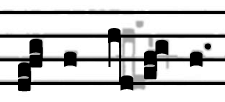
\includegraphics[scale=0.35]{figures/score-detail.png}};
% \node[source] (tasks) at (-2,2.5) {Individual tasks};
  \draw[->,thick] (corpus) -- (tasks);
\node[empty] (decomposition) at (-2,3.75) {Task decomposition};

\node[empty,text width=2.9cm] (engagement) at (2,6.25) {Crowd engagement};
\node[source] (crowd) at (2,5) {Crowd};
\node[source] (orgcrowd) at (2,2.5) {Organized \\crowd};
  \draw[->,thick] (engagement) -- (crowd);
  \draw[->,thick] (crowd) -- (orgcrowd);
\node[empty,text width=2.9cm] (management) at (2,3.75) {Crowd management};

\node[source] (assignment) at (0,0) {Human-checked transcriptions};
\node[source] (quality) at (0,-2.5) {Quality \\control};
\node[source] (output) at (0,-5) {Output};
  \draw[->,thick] (tasks) -- (assignment);
  \draw[->,thick] (orgcrowd) -- (assignment);
\node[empty] (assignment0) at (0,1.25) {Task assignment};
  \draw[->,thick] (assignment) -- (quality);
  \draw[->,thick] (quality) -- (output);
\node[empty] (evaluation) at (0,-1.25) {User/contribution evaluation};
\node[empty,text width=1.8cm] (reward) at (2.95,-2.2) {User reward};
\node[empty] (combination) at (0,-3.75) {Contribution combination};
  \draw[->,thick,rounded corners,awesome] (evaluation) -| (3.8,2) |- (management);
  % \draw[->,thick,rounded corners,dotted] (evaluation) edge[out=0,in=0] (management);
  \draw[->,thick,rounded corners] (output) -| (-4,2) |- (corpus);
  % \draw[-,thick,rounded corners] (output) edge[out=-180,in=-90] (-4,2);
  % \draw[-,thick,rounded corners] (-4,2) edge[out=90,in=-180] (corpus);
  \draw[->,thick,rounded corners,awesome] (evaluation) -| (reward);
  \draw[<->,thick,rounded corners,awesome] (reward) -| (4.2,2) |- (engagement);

\end{tikzpicture}
\end{center}
\caption{A framework for correcting large-scale OMR data with crowdsourcing. Adapted from Kittur et al.~\cite[Fig.~2]{kittur2013}. Workflow- and user-specific challenges are marked in light blue.}
 \label{fig:model}
\end{figure}


% BIBLIOGRAPHY
\clearpage
\phantomsection
\addcontentsline{toc}{chapter}{Bibliography}
\bibliography{crowds}
\bibliographystyle{jasaauthyear}


\end{document}
